\section{Method and Theory}\label{sec:method_theory}
In this chapter we give an overview of the theory and methods which are used throughout this thesis. We begin in Section \ref{sec:cmd_theory} with the description of the stellar population of a \ac{GC}. We introduce the formulas which we will use to investigate \acp{GC} in phase space by analysing the stellar kinematic profiles (such as velocity dispersion and anisotropy profiles, Section \ref{sec:kin_prof_theory}) and the spatial distribution of stars (density profiles and potential, Sections \ref{sec:density} and \ref{sec:poisson}). In Section \ref{sec:other_pot}, we introduce different potential models. In the next Section \ref{sec:iof} we define orbits and their classical integrals of motion. After explaining the benefit of the effective potential in Section \ref{sec:pot_eff}, we show how we calculate the actions as best choice of integrals of motions (Section \ref{sec:actions}). Then we describe the numerical way of calculating orbits (Section \ref{sec:num_int}) for which we also give some examples. If not stated otherwise all integrals of motions are given as specific quantities which means they are given in units of the mass of the star.
\subsection{Stellar population in globular clusters}\label{sec:cmd_theory}
The typical stellar population of a \ac{GC} can be visualised in a \ac{CMD}. We show in Figure \ref{fig:cmd} an example of a \ac{CMD} extracted from one of our simulations (SIM 1, described in Section \ref{sec:description}). In this \ac{CMD} the absolute V-band magnitude is plotted against the B-V color. The color code indicates the mass of the stars. 
\begin{figure}[htbp]
\centering
	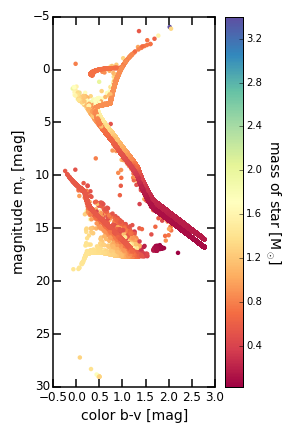
\includegraphics[width=0.7\textwidth]{Plots/color_magnitude_diagram.png}
	\caption{Color magnitude diagram of SIM 1 (see Section \ref{sec:description}). The absolute V-band magnitude versus the color B-V gives us an overview of the stellar population of this \ac{GC}. The stars are color coded by their masses. Since there is only one binary system having a mass of \unit[3.4]{M$_\odot$} and the next heavier object having a mass of \unit[2.4]{M$_\odot$} we set the upper limit of the color at the second highest mass. On the main sequence there are two branches. The brighter and redder sequence is caused by binary systems. Following the main sequence there is the turn-off. Bluewards of the main sequence turn-off point blue struggler stars are located. Redwards of the turn-off there is the sub giant branch followed by the red giant branch. The most luminous stars are situated on the early asymptotic giant branch. At a absolute magnitude of zero there is the horizontal branch where stars burn He quiescently. Below  the main sequence and blue stragglers the white dwarfs are located. Having nearly no luminosity dark stellar remnants are situated at the bottom of the \ac{CMD}.}
	\label{fig:cmd}
\end{figure}
The position of a star in the \ac{CMD} can be interpreted as its evolution stage. If the \ac{GC} was indeed a \ac{SSP}, i.e. all stars had the same age and metallicity, the distribution of stars in the \ac{CMD} would be a function of the stellar mass only ("isochrone"), with more massive stars being in a later evolutionary stage. Most of the stars are still on the main sequence and they are characterized by hydrogen fusion in their cores. There are two main sequence lines one upon the other. These occur due to binary systems whose flux is given by the sum of the single fluxes of the single components, and therefore appear redder and more luminous. These binary systems represent about \unit[7.5]{\%} of the stars in this \ac{GC} simulation. The turn-off point describes the moment in the evolution of the star, when hydrogen in its core is exhausted and it evolves away quickly from the main sequence towards the red giant branch. The position of the main sequence turn-off depends on the age of the system and therefore can be used as an indicator to determine the age of the cluster by comparing it to theoretical isochrones.  
\par Bluewards of this turn-off point, following the trend of main sequence stars, there are the so called "blue straggler" stars which are remnants of stellar collisions or interacting binaries \citep[p.628]{2008gady.book.....B}. Continuing from the turn off point there are the sub giant and the red giant branch consisting of stars still fusing hydrogen but only in a shell surrounding a degenerate helium core. They are inflated with a radius much higher than the main sequence stars but have a much lower surface temperature. On the upper part of the red giant branch lies the horizontal branch. Its stars burn helium in their core and hydrogen in a surrounding shell. On the early asymptotic giant branch following the horizontal branch the stars are burning hydrogen in outer shells helium in inner shells. These are the brightest stars of a \ac{GC} \citep[p.476-477]{2006ima..book.....C}. In the lower left corner white dwarfs are located. They are stellar remnants which have burnt all of their resources. In a typical \ac{GC} dark stellar remnants like stellar black holes and neutron stars are present but not visualised in the \ac{CMD}. In this \ac{CMD} we see them at the bottom of the figure. 
\subsection{Kinematic profiles of globular clusters}\label{sec:kin_prof_theory}
\par The stellar velocity dispersion quantifies the spread of different velocities stars can have at given positions. With the actual velocity \(\mathrm{v_i}\) of the i-th star, \(\left\langle \mathrm{v}\right\rangle\) specifying the mean of the velocities of all considered N stars and the second velocity moment (with the n-th velocity moment given by
\(
\mathrm{\left\langle \mathrm{v^n}\right\rangle=\frac{1}{N}\sum_{i=1}^Nv_i^n}
\)) we can calculate the velocity dispersion as the standard deviation of the velocity distribution: 
\begin{equation}\label{eq:vel_disp}
\sigma_\mathrm{i}(\mathrm{r})\equiv\sqrt{\left\langle(\mathrm{v_i}(\mathrm{r})-\langle \mathrm{v_i}(\mathrm{r})\rangle)^2\right\rangle}=\sqrt{\left\langle \mathrm{v_i}(\mathrm{r})^2\right\rangle-\langle \mathrm{v_i}(\mathrm{r})\rangle^2} \qquad\qquad \mathrm{i=r,\theta,\phi}.
\end{equation}  For a spherical system it is best to calculate them with respect to the spherical coordinates, i.e. \(\mathrm{v_r,v_{\theta},v_{\phi}}\). If the \ac{GC} contains an \ac{IMBH} the velocity dispersion towards the centre is expected to increase. 
\par The preferred direction of the motion of stars can be related to an anisotropy parameter. In a spherical system we compare the motions of the stars in radial direction to the motions in spherical shells (tangential direction) at the given distance of the star. The velocity dispersions of motions are described by Equation \eqref{eq:vel_disp}. To quantify the anisotropy of the system we use the anisotropy parameter \(\beta\) 
\begin{equation}\label{eq:anisotropy}
\mathrm{\beta(r)\equiv1-\frac{\sigma_\theta ^2(r)+\sigma_\phi ^2(r)}{2\sigma_r ^2(r)}}
\end{equation} taken from \citet[eq. 4.61]{2008gady.book.....B}. The numerator describes the velocity dispersion on the spherical shell while the denominator is given by the squared radial dispersion. If \(\beta\) is positive the anisotropy is radial i.e. the velocity dispersion is larger in radial direction than in tangential direction, if it is negative the anisotropy is tangential and if \(\beta\approx0\) then the system is isotropic, that means the stars have random motions in all directions at the same rate. 
\subsection{Density and potential}\label{sec:dens_pot_theory}
\subsubsection{Density of a collisionless stellar system}\label{sec:density}
\acp{GC} are classical examples for quasi-collisional stellar systems, i.e. the motions are dominated by two-body interactions.To allow for an investigation of the orbits the stars are \emph{currently} on, we assume that a star only feels the gravitational forces generated by a smooth overall stellar density distribution, i.e. we assume the system to be collisionless at the moment of our investigation. This is approximately motivated by the fact that the dynamical time of a cluster is always shorter than the relaxation time \(\mathrm{T_{dyn} < T_{relax} < T_{ageGC} \equiv T_{Hubble}}\). \(\mathrm{T_{dyn}}\) is approximated by the time of a star to go from one side of the cluster to the other. This takes approximately \unit[10\(^5\)]{yr}. The relaxation time is the time needed to redistribute energies of the stellar encounters and takes about \unit[10\(^7\) - 10\(^9\)]{yr}. The age of the \acp{GC} is approximately the Hubble time which is the age of the universe (\unit[10\(^{10}\)]{yr}). \(\mathrm{T_{dyn} < T_{relax}}\) motivates the collisionless approximation while t\(\mathrm{T_{relax} < T_{ageGC} \equiv T_{Hubble}}\) is telling us that a \ac{GC} has lived for several relaxation times, therefore two-body interaction had time to act. That means that the system is collisional in the long term, see also \citet[p.555]{2008gady.book.....B} and \citet{2012MNRAS.423.3589W}. 
\par We calculate the mass density of the \acp{GC} by binning the masses on logarithmic equally distributed shells with shell boundaries at $\mathrm{r'_i}$
\begin{equation}\label{eq:density}
\rho_\mathrm{i}=\frac{\sum_\mathrm{k}\mathrm{M_k}}{\mathrm{V(r'_{i+1}-r'_i)}}=\frac{3}{4\pi}\frac{\sum_\mathrm{k}\mathrm{M_k}}{\mathrm{r'_{i+1}^3-r'_i^3}}
\end{equation} 
with the mass m$_\mathrm{k}$ of k-th star, at radius r$_\mathrm{k}$ where  $\mathrm{r'_i=r_k=r'_{i+1}}$  over a volume V which is taken from the radius of the inner shell \(\mathrm{r'_{i}}\) and the radius of the outer shell \(\mathrm{r'_{i+1}}\). We set $\rho_\mathrm{i}\equiv\rho(\mathrm{r_i})$ with r$_\mathrm{i}$ as mean of all r$_\mathrm{k}$.

\subsubsection{Generating the potential from Poisson's equation}\label{sec:poisson}
If the system is spherical symmetric the potential and force depend only on the distance from the centre r. Under the condition that the system is collisionless, the potential \(\Phi\) can be derived from the Poisson's equation \begin{equation}\label{eq:Poisson}
\mathrm{\Delta\Phi(r)=4\pi G \rho(r)}
\end{equation}
with the gravitational constant G = \unitfrac[\(6.674\cdot10^{-11}\)]{\(\mathrm{m}^3\)}{\(\mathrm{kg\ s}^2\)} \citep{2015arXiv150707956M} and the density \(\rho\) depending only on the distance to the centre as well. In general, one can use the Poisson's equation for every system but then it is depending on the position vector \(\vec{\mathrm{x}}\). 
\par Due to the spherical symmetry the potential can be calculated by 
\begin{equation}\label{eq:numerical_poisson}
\mathrm{\Phi(r)=-\frac{G}{r}\int_0^r{\mathrm{d}M(r')}-G\int_r^{\infty}{\frac{\mathrm{d}M(r')}{r'}}=-4\pi G\left[\frac{1}{r}\int_0^r\mathrm{d}r'r'^2\rho(r')+\int_r^{\infty}\mathrm{d}r'r'\rho(r')\right]}
\end{equation} with dM describing the mass of spherical shells as proved by \citet[eq. 2.28]{2008gady.book.....B}. 
\par To numerically calculate the integrals of Equation \eqref{eq:numerical_poisson} from the interpolated density in Section \ref{sec:density} we use the Gauss-Legendre quadrature 
\begin{equation}\label{eq:Gauss-Legendre}
\mathrm{\int_a^b f(x)dx \approx \frac{b-a}{2}\sum_{i=1}^n w_i f\left(\frac{b-a}{2}x_i+\frac{a+b}{2}\right)}
\end{equation} where the points \(\mathrm{x_i}\) and the weights \(\mathrm{w_i}\) are derived from the Legendre polynomials and a and b are the integration limits. This gives us the numerical formula for the potential 
\begin{equation}\label{eq:numerical_potential}
\begin{aligned}
\mathrm{\Phi(r)= }& \mathrm{-4\pi G \cdot \frac{1}{2}\sum_{i=1}^n  w_i\left(\frac{r}{2}x_i+\frac{r}{2}\right)^2\rho\left(\frac{r}{2} x_i+ \frac{r}{2}\right) }\\
& \mathrm{-4\pi G\cdot\frac{\infty-r}{2}\sum_{i=1}^n w_i\left(\frac{\infty-r}{2} x_i +\frac{\infty+r}{2}\right)\rho\left(\frac{\infty-r}{2} x_i +\frac{\infty+r}{2}\right)}
\end{aligned}
\end{equation}
\subsubsection{Other potential models}\label{sec:other_pot}
One of the most simple potentials is the Kepler potential. It describes the potential given by a point mass M
\begin{equation}\label{eq:kep_pot}
\mathrm{\Phi(r)=-\frac{GM}{r}}
\end{equation}  taken from \citet[eq. 2.34]{2008gady.book.....B}. The potential generated by the \acp{IMBH} can be described  as Keplerian. 
\par Another description of spherical systems is given by the Plummer model. It is based on the assumption that the density is nearly constant in the centre and equals zero at large radii. The given potential is 
\begin{equation}\label{eq:Plum_pot}
\mathrm{\Phi(r)=-\frac{GM}{\sqrt{r^2+b^2}}}
\end{equation}
\citep[eq. 2.44a]{2008gady.book.....B} where M is the total mass of the system and b is the Plummer scale length. In \citet{1911MNRAS..71..460P} this potential is used to describe observations of \acp{GC}. The corresponding density to this model is given by \citet[eq. 2.44b]{2008gady.book.....B}
\begin{equation}\label{eq:Plumm_dens}
\mathrm{\rho(r)=\frac{3M}{4\pi b^3}\left(1+\frac{r^2}{b^2}\right)^{-\frac{5}{2}}.}
\end{equation} 
\par Another potential, which is the most general potential for which the actions (see Section \ref{sec:actions}) can be calculated exactly and analytically without the use of an integration, is the isochrone potential
\begin{equation}\label{eq:isochr_pot}
\mathrm{\Phi(r)=-\frac{GM}{b+\sqrt{b^2+r^2}}}
\end{equation} 
\citep[eq. 2.47]{2008gady.book.....B}. The Kepler potential is a special case of the isochrone potential with b$=0$. 
\subsection{Orbits and integrals of motion}\label{sec:orbit_int_of_motion_theory}
\subsubsection{Classical integrals of motion in spherical potentials}\label{sec:iof}
If a tracer particle, e.g. a star, moves freely in a gravitational potential generated by a mass distribution its path in 6D position-velocity space (\(\vec{\mathrm{x}}(\mathrm{t}),\vec{\mathrm{v}}(\mathrm{t})\)) is called "orbit".
The way in which positions and velocities along the orbit are linked contains information about the potential. With Newton's 2nd law we get the connection between potential \(\Phi(\vec{\mathrm{x}})\) and acceleration \(\vec{\mathrm{a}}(\vec{\mathrm{x}})\) which the star of mass m experiences which is 
\begin{equation}\label{eq:Newton}
\vec{\mathrm{F}}(\vec{\mathrm{x}})=-\mathrm{m}\nabla\Phi(\vec{\mathrm{x}})=\mathrm{m}\cdot\vec{\mathrm{a}}(\vec{\mathrm{x}}).  
\end{equation}
Here \(\vec{\mathrm{F}}\) is the force at given position \(\vec{\mathrm{x}}\).
\par Beside the description of orbits in the 6D position velocity space, orbits can be described by integrals of motion which are constant along an unperturbed orbit. A spherical potential allows four conserved quantities, e.g. the classical integrals of motions, which are the energy and the three components of the angular momentum. That restricts the orbits in spherical potentials to lie in a plane. The (specific) energy is given by the sum of the kinetic energies in the 3D velocity space and the potential energy:
\begin{equation}\label{eq:energy}
\mathrm{E(r)=\frac{v_x(r)^2+v_y(r)^2+v_z(r)^2}{2}+\Phi(r)}.
\end{equation}
The total (specific) angular momentum
\begin{equation}\label{eq:total_ang_mom}
\vec{\mathrm{L}}=\vec{\mathrm{x}}\times\vec{\mathrm{v}}=\sqrt{\mathrm{L_x^2+L_y^2+L_z^2}}
\end{equation}
can be written as superposition of the angular momenta in each direction which are given by 
\begin{equation}\label{eq:ang_mom}
\mathrm{L_k=\varepsilon_{klm}x_l v_m}
\end{equation}
where \(\mathrm{\varepsilon_{klm}}\) is the Levi-Civita symbol.  
\par If an orbit is perturbed its integrals of motion can vary and evolve a time dependency. There are physical reasons for perturbations (e.g. scattering due to two- and three-body interactions when passing by other stars, stellar binaries or the \ac{IMBH}); in computer simulations there can be in addition also numerical fluctuations of the orbits close to the \ac{IMBH}. We assume that the stars move along unperturbed orbits.
\subsubsection{The effective potential}\label{sec:pot_eff}
The effective potential \(\mathrm{\Phi_{L}(r)}\) (see Figure \ref{fig:pot_eff_theory}) combines the effects of gravitational force and centrifugal force acting on a star moving with given angular momentum L in a gravitational potential \(\Phi(\mathrm{r})\):
\begin{equation}\label{eq:eff_pot}
\mathrm{\Phi_L(r)=\Phi(r)+\frac{L^2}{2r^2}}.
\end{equation} 
which is dependent on the centrifugal potential \(\mathrm{L^2/2r^2}\) (taken from \citealp[p. 59, eq. 6.27]{bartelmann}). The centrifugal potential describes the energy that star has due to its rotation. If the orbit is unbound its total energy is larger than its effective potential at large radii. A star on a bound orbit has a total energy which is smaller than the effective potential everywhere except between a certain minimum and maximum radius. 
\begin{figure}[htbp]
\centering
\subcaptionbox{General potential of a central field. The black line is the gravitational potential, the effective potential is given by the yellow line and the centrifugal potential by the red line. If the effective potential is positive the object is unbound while having a negative potential the object moves on a bound orbit. The points where the effective potential equals the total energy are the peri- and apocentre (r\(_1\) and r\(_2\)) of the orbit. The point with the lowest effective potential is the guiding-star radius. This is the distance a star with given angular momentum would have on a circular orbit. \citep[p.59]{bartelmann}\label{fig:eff_potential_bartelmann}}{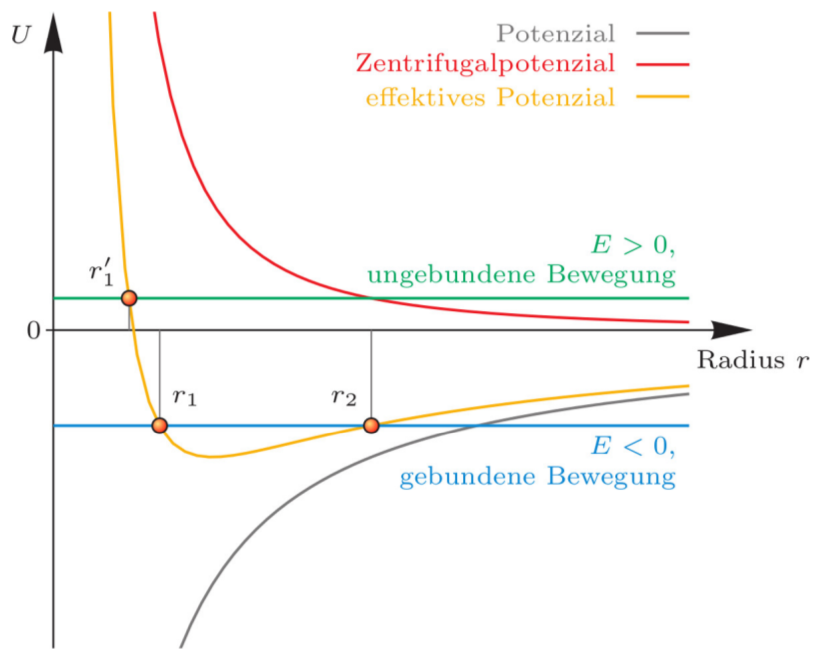
\includegraphics[width=0.475\textwidth]{Plots/eff_potential_bartelmann.png}}
\hfill
\subcaptionbox{Determination of pericentre, apocentre and guiding-star radius given by Equation \eqref{eq:root_pot_eff}. Where the difference between effective radius and total energy is zero (red dashed line), are the peri- and the apocentre of the star (magenta and black lines) and the minimum of the effective potential (green line) is the guiding-star radius. This figure shows function \ref{eq:root_pot_eff} for a star in SIM 1 (see Section \ref{sec:description}) with energy E$=$\unitfrac[$-2.7\times 10^{-25}$]{pc$^2$}{s$^2$} and total angular momentum |L|$=$\unitfrac[$5.6\times10^{-13}$]{pc$^2$}{s}.  \label{fig:pot_eff_theory_part}}{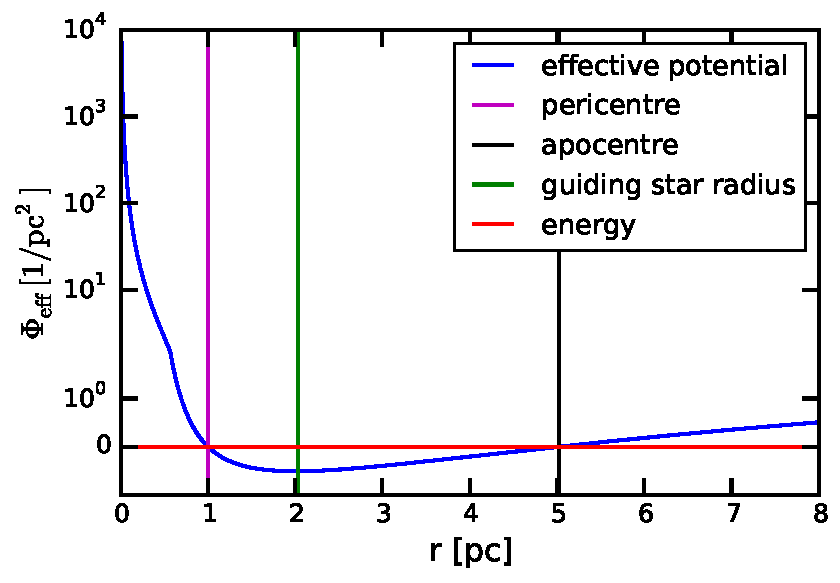
\includegraphics[width=0.475\textwidth]{Plots/pot_eff_theory_part.pdf}}
\caption{Effective potential (Panel (\subref{fig:eff_potential_bartelmann})) and its root to calculate pericentre, apocentre and guiding-star radius (Panel (\subref{fig:pot_eff_theory_part})).}
\label{fig:pot_eff_theory}
\end{figure}

\par These radii where the bound orbit has the smallest and respectively the highest distance to the gravitational centre are called pericentre \(\mathrm{r_{min}}\)  and apocentre \(\mathrm{r_{max}}\).  There the effective potential equals the total energy E since the stars do not have any kinetic energy in radial direction. That results in the following function (see Figure \ref{fig:pot_eff_theory_part}) which is to solve: 
\begin{equation}\label{eq:root_pot_eff}
\mathrm {\Phi(r_0)-E +\frac{L^2}{2r_0^2}=0\Rightarrow\left(\frac{1}{r_0}\right)^2+\frac{2\cdot (\Phi(r_0)-E)}{L^2}=0.}
\end{equation}
r\(_0\) is the solution for peri- and apocentre.
\par The guiding-star radius is the distance at which a star with given total angular momentum would have a circular orbit. This is at the minimum of the effective potential. To get \(\mathrm{r_g}\) we have to solve
\begin{equation}\label{eq:min_pot_eff}
\mathrm{\frac{\partial\Phi_L}{\partial r}=\frac{\partial\Phi}{\partial r}-\frac{L^2}{r^3}=0\Rightarrow r\sqrt{r\frac{\partial\Phi}{\partial r}}-|L|=0}
\end{equation} where \(\mathrm{\sqrt{r\frac{\partial\Phi}{\partial r}}=v_{circ}(r)}\) is the circular velocity. The guiding-star distance is an estimation for the radius where the star is on average. Therefore it can be used to have a better comparison of the positions of the stars in the different simulations since in the snapshots the stars are at a random position on their orbit.

\subsubsection{Actions}\label{sec:actions}
In Section \ref{sec:iof} we introduced the classical integrals of motion. Now we introduce actions which are the best choice of values to describe orbits. Like the classical integrals of motion they are constant over time and orbit. We can combine actions with angle coordinates. The angle coordinates evolve linearly in time while the star moves along the orbit and the actions are the corresponding conjugate momenta. Actions $\vec{\mathrm{J}}$ and angles $\vec{\theta}$ form a set of 6D canonical conjugate coordinates. That means that the transformation from configuration space (\(\vec{\mathrm{x}}(\mathrm{t}),\vec{\mathrm{v}}(\mathrm{t})\)) to action-angle space conserves the phase space volume (i.e. the Jacobian determinant of the transformation is 1). Another reason to have them as best choice is that they have an intuitive physical meaning. They quantify the amount of oscillation along an orbit in the i-direction. Generally they can be calculated by 
\begin{equation}\label{eq:gen_actions}
\mathrm{J_i\equiv\frac{1}{2\pi}\oint_{orbit} p_i\cdot dq_i}
\end{equation} with the spatial coordinate in i-direction \(\mathrm{q_i}\) and the corresponding canonical conjugate momentum \(\mathrm{p_i}\) (if \(\mathrm{p_i}\) is given per unit mass, i.e. is equal to the velocity \(\mathrm{v_i}\), then the radial action is given per unit mass as well). 
\par For most potentials actions cannot be calculated analytically but in spherically symmetric potentials they can be described by relatively straightforward functions. The azimuthal action J\(_\phi\) and the latitudinal action J\(_\theta\) can be evaluated simply. To calculate the radial action J\(_r\) we have to solve an integral numerically. Actions of a spherical potential are found to be 
\begin{align}
\mathrm{J_\phi}&=\mathrm{ L_z}, \label{eq:j_phi} \\\mathrm{ J_\theta}&=\mathrm{ L-|L_z|},  \label{eq:j_theta}\\ \mathrm{J_r}&=\mathrm{ \frac{1}{\pi} \int_{r_{min}}^{r_{max}} \mathrm{d}r \sqrt{2E-2\Phi(r)-\frac{L^2}{r^2}}} \label{eq:radial_action}
\end{align} \citep[p. 221]{2008gady.book.....B}.
The azimuthal action is given by the z-component of the angular momentum which is perpendicular to the z$=0$ plane, i.e. it describes the amount of rotation around the z-axis. The latitudinal action is described by the angular momentum without the component in z-direction. It describes the amount of movement the star performs perpendicular to the z$=0$ plane. The radial action is depending on pericentre and apocentre of the orbit as well as the potential, the total energy and the angular momentum of the orbit. If the radial action is large, then the orbit is either very eccentric and therefore \(\mathrm{r_{max}>>r_{min}}\) or it has a large radial velocity since the integrand equals the radial velocity, as explained in the following. An orbit with $\mathrm{J_r}=0$ is circular since \(\mathrm{r_{max}=r_{min}}\) and $\mathrm{v_r}=0$.
\par We give an heuristic explanation of the formula of the radial action. In the general equation to calculate actions, Equation \eqref{eq:gen_actions}, we set $\mathrm{p_r} = \mathrm{v_r} $, i.e. the velocity in radial direction. We can assume that the spatial coordinate is pointing in r-direction and therefore \(\mathrm{q_r=r}\). In a spherical potential the motions in r,\(\theta\),\(\phi\)-direction are separable \citep[sec. 3.5.2]{2008gady.book.....B}. That allows us to consider the integral in Equation \eqref{eq:gen_actions} (for i$=$r) independent of $\vartheta$ and $\phi$ so that the integral over the whole orbit reduces to a single integration from peri- to apocentre, because the orbit is a closed curve. This leads us to 
\begin{equation}\label{eq:J_r_alpha}
\mathrm{J_r=\frac{2}{2\pi}\int_{r_{min}}^{r_{max}}v_r(r)dr}.
\end{equation}
Now we consider the motion in orbital plane only. We can separate it into the radial motion with given radius r and corresponding velocity v\(_\mathrm{r}\) and into tangential motion with given angle \(\vartheta\) and velocity v\(_\vartheta\). The kinetic energy can then be described as the sum of kinetic energy in radial direction E\(_\mathrm{r}\) and in angular direction E\(_\vartheta\) which is the rotation energy: 
\begin{align}
\mathrm{E_{kin} }&=\mathrm{E_r+E_\vartheta},\\\mathrm{E_r} & \sim \mathrm{ \frac{v_r^2}{2} },\\\mathrm{ E_\vartheta} & \sim \mathrm{ \frac{v_\vartheta^2}{2}\sim \frac{L^2}{2r^2}}. 
\end{align}
We can write the radial energy as sum of the other energies and derive the radial velocity from that:
\begin{align*}
\mathrm{E}& = \mathrm{ E_{kin}+\Phi(r)}\\
\implies \mathrm{E_r} & \sim \mathrm{ E- \Phi(r)-\frac{L^2}{2r^2}}\\
\Leftrightarrow \mathrm{\frac{v_r^2}{2} } & \sim \mathrm{ E-\Phi(r)-\frac{L^2}{2r^2}}\\
\implies \mathrm{v_r} & \sim \mathrm{ \sqrt{2E-2\Phi(r)-\frac{L^2}{r^2}}}.
\end{align*}
We can set this result in the integrand of Equation \eqref{eq:J_r_alpha} which gives us the equation of the radial action. 
\par For the isochrone potential in Equation \eqref{eq:isochr_pot} the radial action given by Equation \eqref{eq:radial_action} reduces to the simple expression 
\begin{equation}\label{eq:isochrone_radial_action}
\mathrm{J_r=\frac{GM}{\sqrt{-2E}} -\frac{1}{2} \left(L+\sqrt{L^2+4GMb}\right)}
\end{equation}
\citep[p.221, eq. 3.225]{2008gady.book.....B}.
\subsubsection{Numerical orbit integration}\label{sec:num_int}
\par To describe the orbit of a star in a potential we need the position and velocity at each time step. For general potentials this has to be calculated numerically. We use the numerical leapfrog method which is a second-order accurate, time reversible, sympletic integrator \citep[p.199/200]{2008gady.book.....B}. Second-order accurate means that the error of the position after one timestep \(\Delta t\) is proportional to the 3rd power of the timestep and sympletic means that it conserves the volume of the phase space. This integrator uses kick steps and drift steps. When doing a kick step the position stays the same and the momentum changes. When doing a drift step the position changes and the momentum stays the same. One variant is the "drift-kick-drift" leapfrog where the steps are calculated as follows:
\begin{equation}\label{eq:drift-kick-drift}
\vec{\mathrm{x}}_{1/2} = \vec{\mathrm{x}}+\frac{1}{2}  \vec{\mathrm{v}}\Delta \mathrm{t} \qquad;\qquad \vec{\mathrm{v}}'=\vec{\mathrm{v}}- \nabla\Phi(\vec{\mathrm{x}}_{1/2})\Delta\mathrm{t} \qquad ; \qquad \vec{\mathrm{x}}' = \vec{\mathrm{x}}_{1/2}+\frac{1}{2} \vec{\mathrm{v}}' \Delta \mathrm{t}
\end{equation} (adapted from \citet[eq. 3.166a]{2008gady.book.....B}).
The second time derivative of \(\vec{\mathrm{x}}\)(t) is the acceleration, which we can assume as constant for small enough timesteps. Integrating the acceleration gives us the velocity at given time t with constant values for the acceleration and velocity. Another integration leads to the position at time t with constant acceleration, velocity and position: \(\vec{\mathrm{x}}(\mathrm{t})=\frac{1}{2}\vec{\mathrm{a}}_0\mathrm{t}^2+\mathrm{v_0t+x_0} \). If we let this position at time t\(_\mathrm{i}\) move for a timestep \(\Delta\)t then we get Equation \eqref{eq:leapfrog_pos}. According to Equation \eqref{eq:Newton} the potential is related to the acceleration by \(\nabla\Phi(\vec{\mathrm{x}})=-\vec{\mathrm{a}}(\vec{\mathrm{x}})\). If the timestep \(\Delta\)t is small enough we can assume that the acceleration is constant for this step and that the acceleration of the half step can be described by the sum of half of the acceleration at the beginning of the step and half of the acceleration at the end of the step. That allows us the following substitution: \(-\nabla\Phi(\vec{\mathrm{x}}_{i/2})=\frac{ \vec{\mathrm{a}}(\vec{\mathrm{x}}_{i+1})+\vec{\mathrm{a}}(\vec{\mathrm{x}}_i)}{2}\) and leads us to Equation \eqref{eq:leapfrog_vel}:
\begin{align}
\mathrm{x_{i+1}} &= \mathrm{x_i+v_i\Delta t+\frac{a(x_i)}{2}\Delta t^2} \label{eq:leapfrog_pos}\\
\mathrm{v_{i+1}} &= \mathrm{v_i+\frac{a(x_{i+1})+a(x_i)}{2}\Delta t}.\label{eq:leapfrog_vel}
\end{align}
We have implemented the leapfrog integrator in the form of Equations \eqref{eq:leapfrog_pos} and \eqref{eq:leapfrog_vel} with Equations \eqref{eq:drift-kick-drift} as fundamental equations of this method.

\par Now we show some examples of different kind of integrated orbits by the leapfrog method in spherically symmetric potentials. We use an isochrone potential in which actions, especially the radial action can be calculated exactly and analytically, see Equations \eqref{eq:j_phi}, \eqref{eq:j_theta} and \eqref{eq:radial_action}. It is also an approximative description of \acp{GC} \citep{2014arXiv1411.4937B}. It is calculated by Equation \eqref{eq:isochr_pot} using the best fit values of the total mass M and the scale length b from fitting the isochrone density profile to the density profile of one of our simulations, SIM 1 (see Section \ref{sec:description}). The best fit parameters are M$=$\unit[1.3$\times10^5$]{M$_\odot$} and b$=$\unit[0.54]{pc}. To get the isochrone potential, integrate the orbits and get the integrals of motion we want to investigate we use galpy, a python package for galactic dynamics from \citealp{2015ApJS..216...29B}. We have implemented this method as well, but use galpy due to its good stability, its faster runtime and its versatility.


\begin{figure}
\centering
\subcaptionbox{{Integrated circular orbit in the z=0 plane.}
\label{fig:galpy_circ_orbit}}{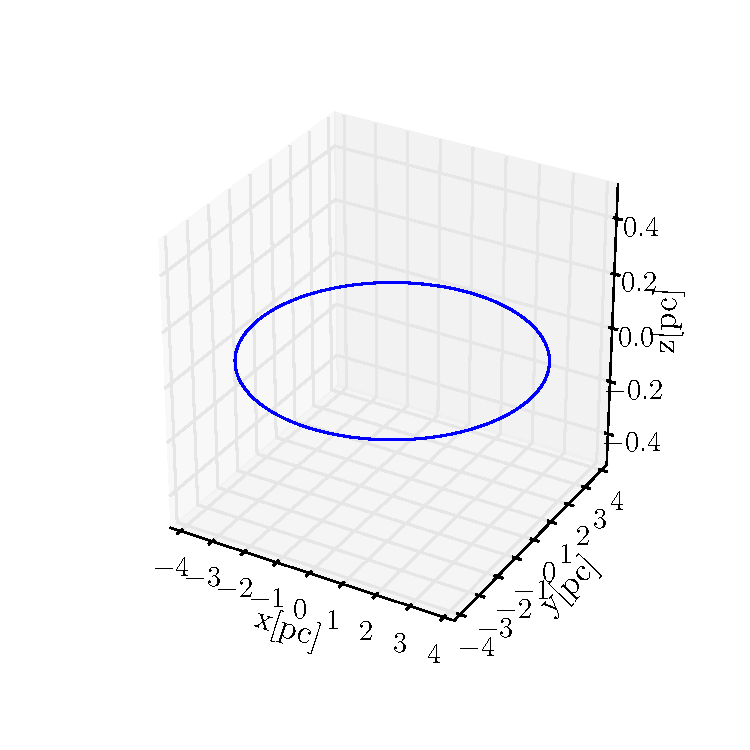
\includegraphics[width=0.3\textwidth]{Plots/galpy_circ_orbit3d.pdf}}
\hfill
\subcaptionbox{{Integrated circular orbit in a random plane.}
\label{fig:galpy_circ_orbit_random_plane}}{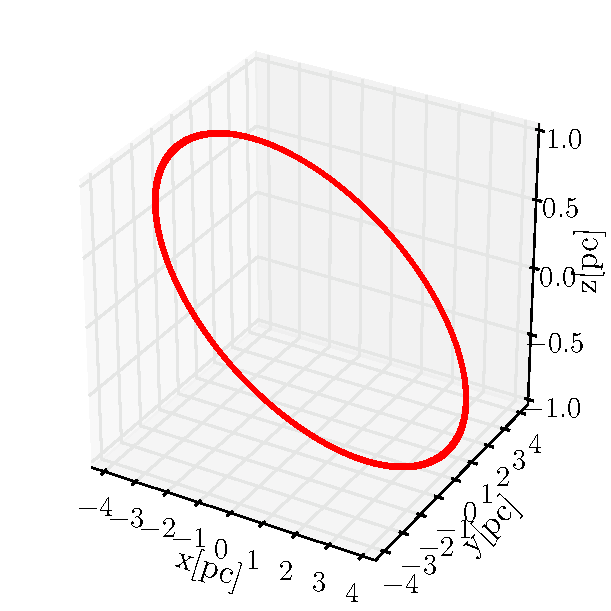
\includegraphics[width=0.3\textwidth]{Plots/galpy_circ_orbit_anyplane_3d.pdf}}
\hfill
\subcaptionbox{{Integrated random orbit in random plane.}\label{fig:galpy_random_orbit}}{{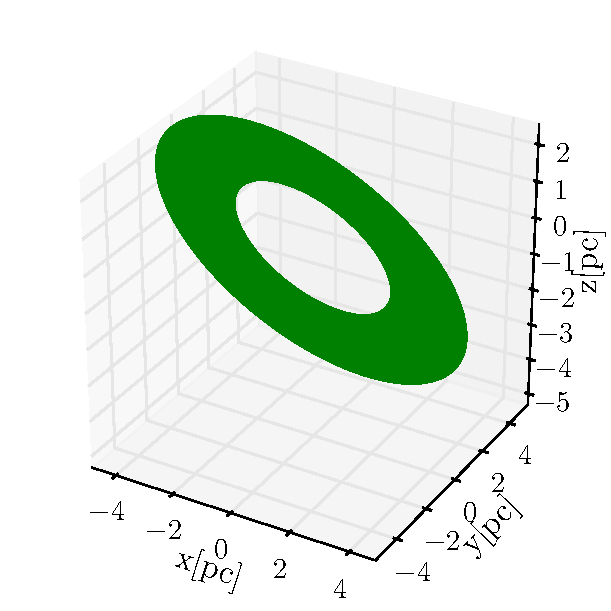
\includegraphics[width=0.3\textwidth]{Plots/galpy_random_orbit3d.pdf}}}

\caption{Three examples of orbits integrated with the leapfrog integrator using galpy. The initial conditions are given in Table \ref{tab:overview_orbits}.}
\label{fig:orbits}
\end{figure}

All three orbits of Figure \ref{fig:orbits} move in a plane, because the angular momentum $\vec{\mathrm{L}}$ is conserved. For a long enough integration time the orbit completely fills the annulus between its pericentre and apocentre. The orbit in Panel (\subref{fig:galpy_random_orbit}) has a radial action $\mathrm{J_r>0}$ (see Figure \ref{fig:orbits}). The circular orbits in Panels (\subref{fig:galpy_circ_orbit}) and (\subref{fig:galpy_random_orbit}) have no inward or outward motion and $\mathrm{J_r=0}$. In Panel (\subref{fig:galpy_circ_orbit_random_plane}) the plane of the orbit is rotated with respect to the z$=0$ plane.  
We choose following initial conditions for position, velocity and therefore the radial action:

\begin{table}[htbp]
\centering
\begin{tabular}{ c | c | c | c | c | c | c | c }
& r [pc] & z [pc] & $\phi$ [pc]& v$_\mathrm{r}$ [pc] & v$_\mathrm{T}$ [pc] & v$_\mathrm{z}$ [pc] & J$_\mathrm{r}$ \unitfrac{pc km}{s}\\
\hline			
Panel (\subref{fig:galpy_circ_orbit}) & 4.13 & 0.0 & 0.0 & 0.0 & 10.15 & 0.0 & 0.0\\
Panel (\subref{fig:galpy_circ_orbit_random_plane})& 4.13 & -0.83 & 0.0 & 0.0 & 10.15& 0.0 & 0.0\\
 Panel (\subref{fig:galpy_random_orbit}) & 4.13 & -2.07& 0.0& 2.03 & 8.12 & -2.03 & 0.85\\


\end{tabular}
\caption{Overview of the initial conditions used for the orbit integration. All position coordinates are given in pc and the velocity coordinates are given in \unitfrac{km}{s}. The radial action J$_\mathrm{r}$ is given in \unitfrac{pc km}{s}. The radius is given by r, the height by z and the angular coordinate by $\phi$. The velocities are given by v$_\mathrm{r}$ in the radial direction and  v$_\mathrm{T}$ and v$_\mathrm{z}$ as tangential velocities.}
\label{tab:overview_orbits}
\end{table}

